
\chapter{背景知识}

本章介绍了云边协同和边缘端节点监测技术两个方面的背景知识。首先,介绍了云边协同的基本概念,详细阐述了云边协同中推理服务的供应问题,并且提出本文原型系统的底层框架 KubeEdge。其次,概述了边缘端节点监测技术,包括边缘端节点推理能力监测技术和通信监测技术。

\section{云边协同计算范式}

云边协同是在云计算和边缘计算两种典型计算范式的基础上发展起来的,旨在充分发挥两者的优势,以实现低延迟、高可用的数据处理和服务提供\cite{李波2021基于软件定义网络的云边协同架构研究综述}。在传统的云边协同架构中,当请求在终端设备上产生时,轻量级请求通常可以直接由设备本地处理,而较复杂的请求则需要分发到附近的边缘服务器进行处理。边缘服务器处理完成后,结果会立即返回终端设备,从而保证较低的响应延迟。然而,边缘服务器的计算和存储能力有限,通常只能支持有限的应用和功能,因此对于无法快速处理的请求,最终将被转发到云计算中心进行处理。云边协同的架构通常可以分为“端-边-云”三个层级\cite{mao2017survey,satyanarayanan2017emergence,吴大鹏2018端},如图 \ref{fig:2-1云边端架构} 所示:

\begin{itemize} 
\item \textbf{端层(End Layer)}:位于网络的最前端,包括物联网设备、传感器及终端用户设备。端层负责直接与现实世界交互,进行数据采集和初步处理,如数据过滤或简单分析。同时,端层设备通过无线或有线连接与边层节点进行数据传输和指令通信,确保信息的及时传递与响应。
\item \textbf{边层(Edge Layer)}:由边缘服务器、网关及边缘计算节点等设备组成,处于端层与云层之间。边层节点靠近数据源,具备一定计算和存储能力,能够对来自端层的数据进行实时处理与分析,执行较为复杂的计算任务,并在必要时与云层节点进行通信,以协调更大规模的资源和服务。
\item \textbf{云层(Cloud Layer)}:通常由大型云计算数据中心构成,提供强大的计算、存储和网络资源。云层节点负责处理需要大规模计算能力的任务,进行深度数据分析和机器学习模型训练,并管理和存储海量数据。云层还支持跨地域的资源调度和服务集成,提供全局性的决策支持和业务逻辑。
\end{itemize}

\begin{figure}[ht]
  \centering
  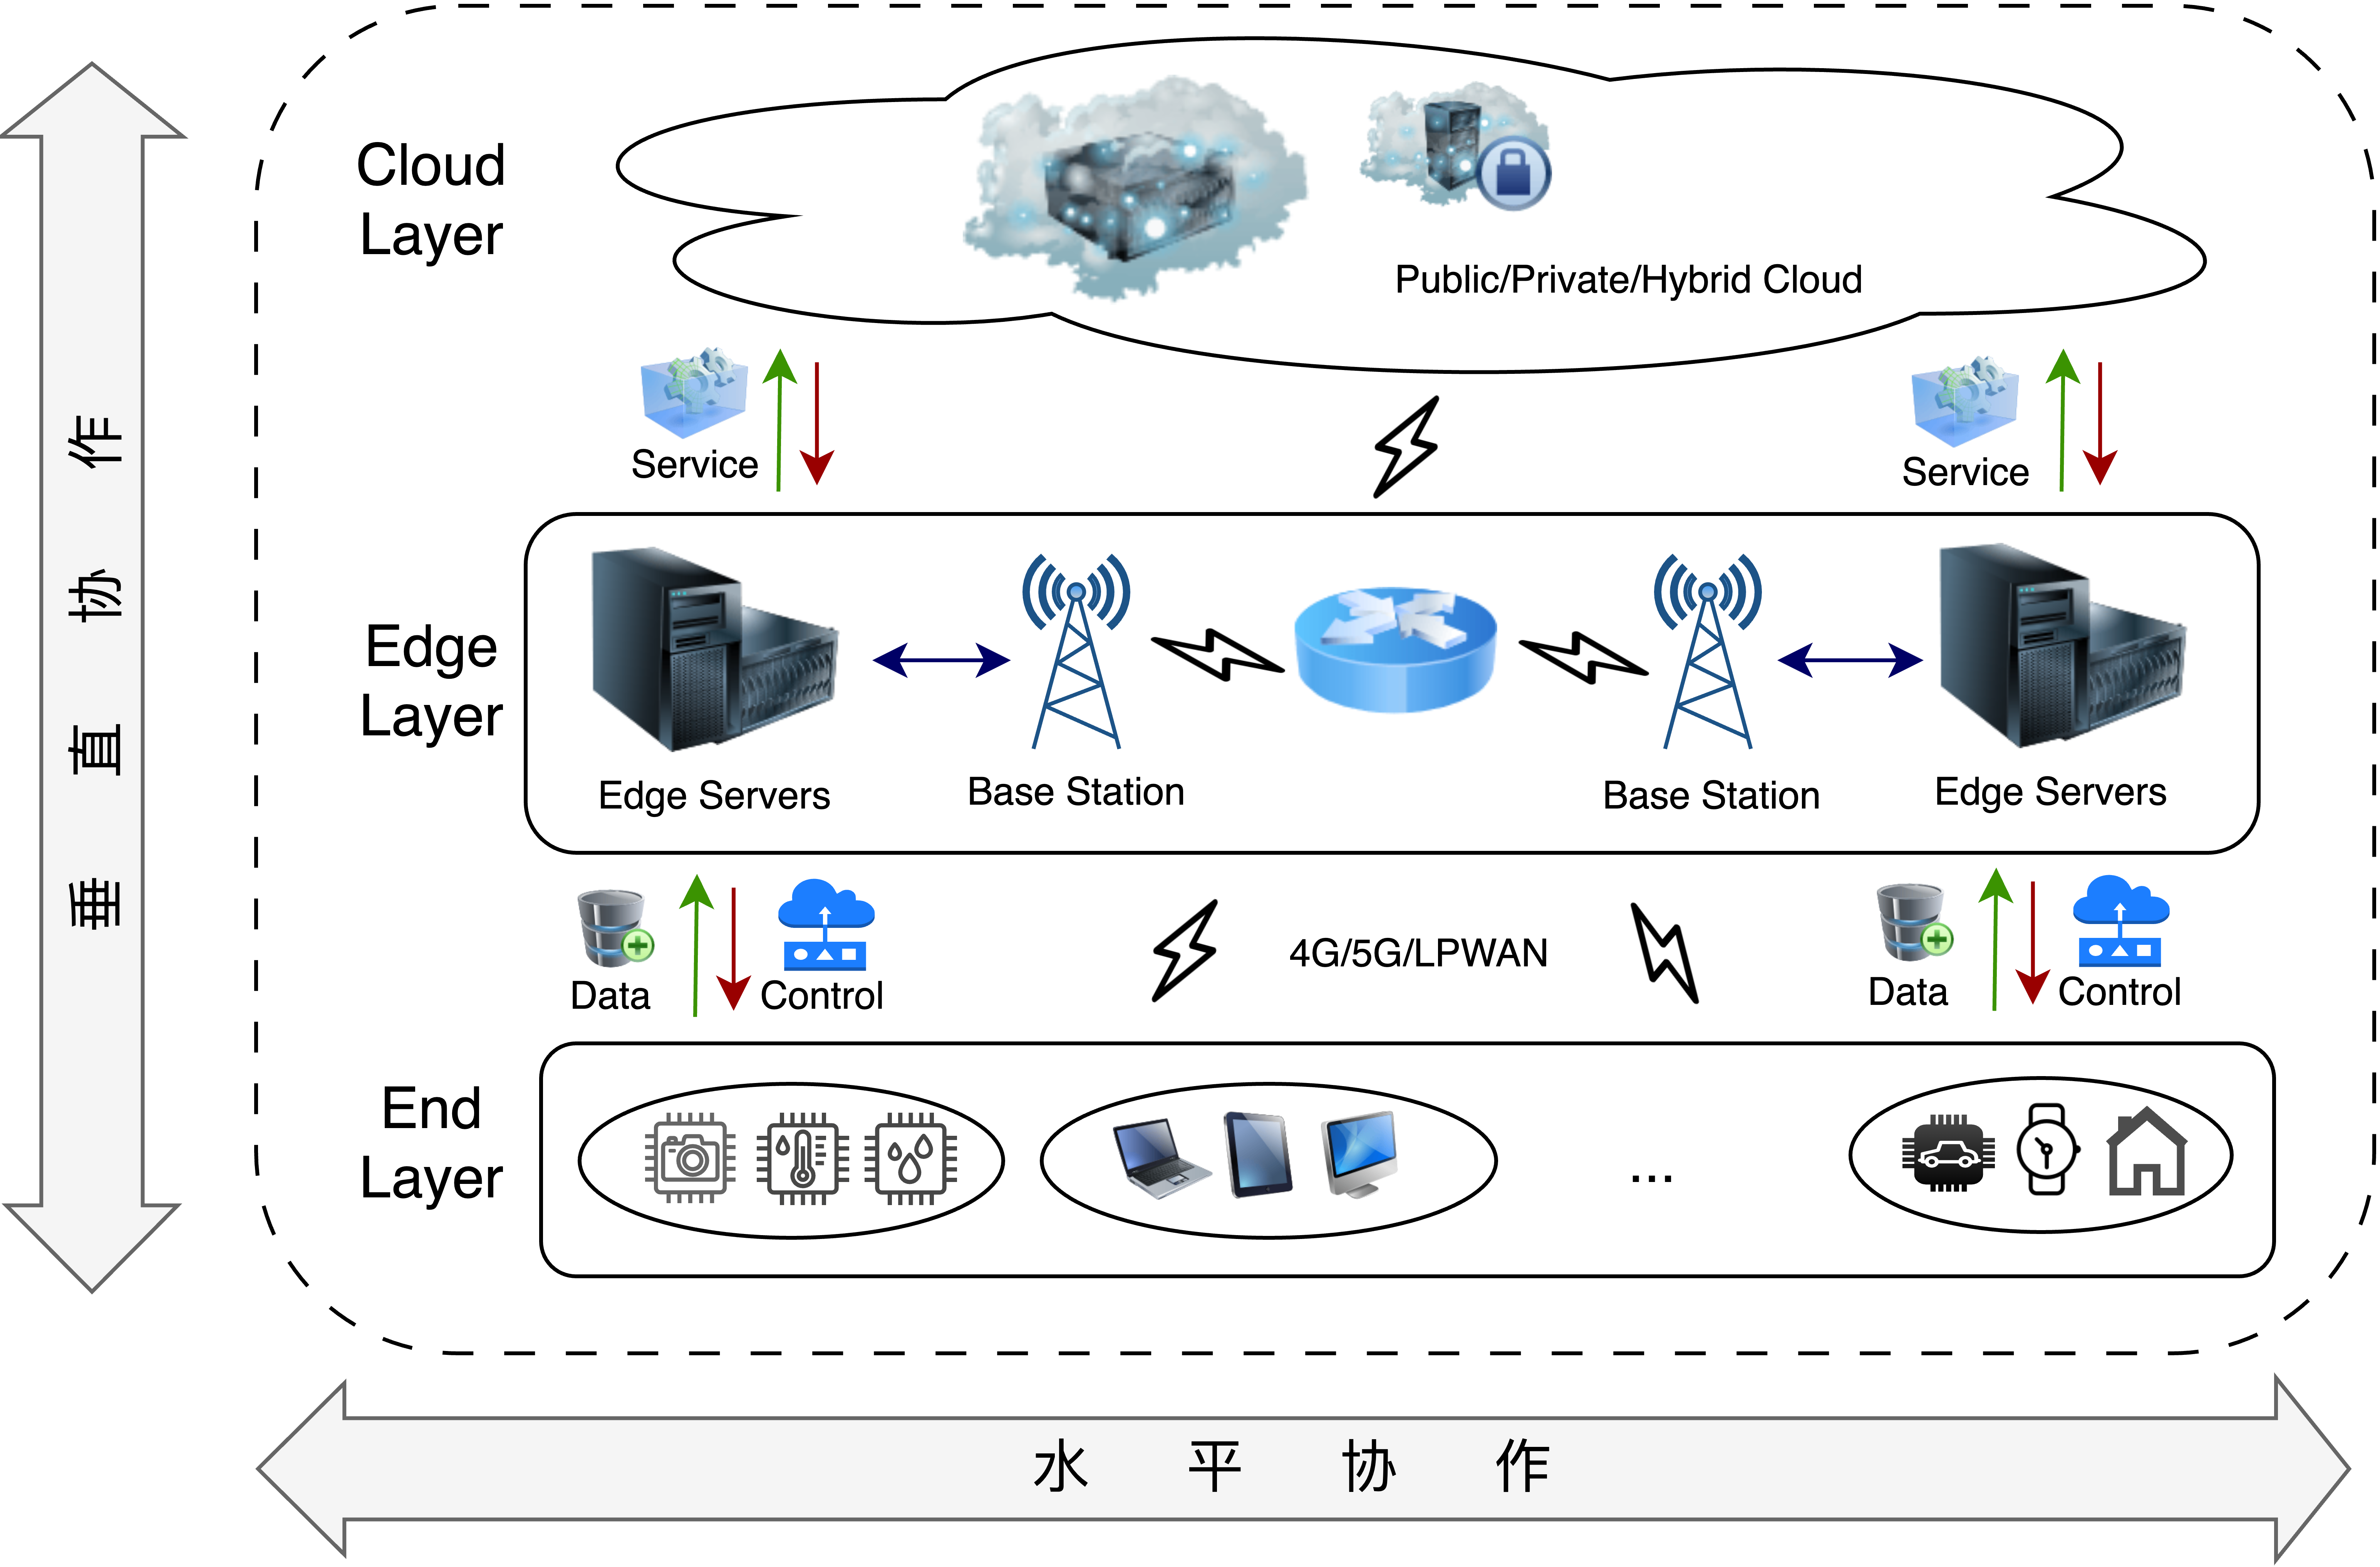
\includegraphics[width=\linewidth]{pics/2-1云边端架构.png}
  \caption{云边协同的“端-边-云”三层架构}
  \label{fig:2-1云边端架构}
\end{figure}

部分研究\cite{lane2016deepx,teerapittayanon2017distributed,liu2023adaptive}进一步指出,具有初步计算能力的端层设备也可与边缘服务器协同完成推理任务。为便于论述,本研究将这类端层设备与边层节点统一视为“边缘端”,而将云层节点称为“云端”。通过这种分层架构,云边协同能够有效利用不同层级的计算资源,从垂直和水平两个角度进行资源优化\cite{dupont2017edge,li2020elastic}。垂直优化指的是在“端-边-云”各层之间进行资源分配与优化,需要将云端和边缘端的硬件资源进行虚拟化抽象,并依据应用需求统一管理与分配。基于应用特性,计算任务可以被合理地部署在云端或边缘端,同时在层次之间需优化传输路径协议,并采取加密等手段保障数据安全。水平优化则关注同一层级内的资源协同,特别是边缘节点之间的协作计算。通过任务分割和并行计算,水平优化能够提升计算效率。通过动态监测边缘节点的负载情况,系统能够将计算任务合理分配到负载较轻的节点,进而利用负载均衡算法优化资源的使用,提升整体计算性能。

\subsection{云边协同中推理服务的供应现状}

深度学习模型通过训练实现推理功能,即通过学习大规模数据提取特征并优化参数,从而在推理阶段快速生成预测结果。模型训练因其计算和 I/O 密集性长期是研究优化的重点,而推理虽无需复杂迭代算法,通常被认为较为简单。然而,随着深度学习应用的快速发展,推理不仅需要满足更高的实时性要求,还需应对海量传感设备带来的急剧增长需求,这对系统性能和资源分配提出了严峻挑战。

目前,深度学习推理服务的供应主要有两种方式:一是通过边缘设备运行简单模型提供服务;二是依托远程云基础设施,通过“机器学习即服务”(MLaaS)平台运行复杂模型,以高吞吐量支持推理。然而,这两种方式在某些场景下存在局限性——边缘设备的模型难以满足精度需求,而云服务则无法达到严格的低延迟要求。在此背景下,云边协同计算通过结合云与边缘的优势,利用智能资源编排和优化调度机制,在性能与延迟之间实现有效权衡,在深度学习模型调度中发挥了重要作用。

尽管如此,目前大多数推理服务解决方案,如 TensorFlow Serving\cite{olston2017tensorflow} 和 Azure ML\cite{chappell2015introducing},主要面向云端推理服务的供应问题。然而,这些解决方案在应对复杂推理需求和多样化应用时存在一定局限性,尤其是在延迟和吞吐量方面。为了解决这些问题,Crankshaw 等人\cite{crankshaw2017clipper} 提出了 Clipper 系统。Clipper 通过实现预测缓存,减少了频繁查询带来的延迟和系统负载,并利用自适应批处理技术,根据模型容器的延迟配置文件动态调整批处理大小,从而优化了吞吐量与延迟之间的平衡。Clipper 还通过模型抽象层简化了不同机器学习框架之间的差异,使得开发者能够专注于模型的部署和优化,而无需关注底层框架的选择。在此基础上,Crankshaw 等人\cite{crankshaw2020inferline}提出了 InferLine,一个用于配置和管理机器学习推理管道的系统。InferLine 专注于在异构并行硬件上以低成本满足端到端延迟要求,系统通过为每个模型创建性能配置文件并估算管道的端到端延迟,优化了管道的资源分配。它还能根据实际工作负载的变化,动态调整管道配置,在负载增加时自动扩展副本数,并在负载减小时根据最小供应比率缩减副本数,从而确保系统始终满足延迟和吞吐量要求。此外,Mao 等人\cite{mao2019learning} 提出了名为 Decima 的架构,基于强化学习调度策略,可以在无需人工输入复杂调度算法的情况下,根据不同工作负载和环境条件自动学习最优策略,从而提高集群资源的利用率。然而,以上这些解决方案主要解决了云端推理服务的供应问题,并未充分考虑边缘端节点的特殊需求,尤其是在小型集群和网络延迟至关重要的地理分布式基础设施中。例如,这些方案都没有考虑不同计算节点之间的网络延迟,而在云端部署环境中,网络延迟往往可以忽略不计。

针对边缘端推理服务供应问题,目前相关研究仍然较少。一些研究提出了模型拆分技术,通过将深度学习模型的执行分布到多个离散计算单元上,以适应移动硬件平台的资源限制。Lane 等人\cite{lane2016deepx} 提出了 DeepX 框架,专注于优化深度学习模型在移动设备上的推理性能。该框架通过运行时层压缩(RLC)和深度架构分解(DAD)两种核心算法有效缓解了移动设备资源受限的难题。RLC 方法利用奇异值分解(SVD)对模型权重进行压缩,显著降低计算量和内存占用,同时通过引入估计器控制压缩程度,确保模型准确性保持在可接受范围内。DAD 方法则通过将复杂的深度模型分解为多个单元块,并将其分配到本地和远程处理器上,最大化资源利用效率。在推理过程中,这些单元块的计算结果会被重组,生成最终的预测输出。此外,Teerapittayanon 等人\cite{teerapittayanon2017distributed} 提出了分布式深度神经网络(DDNN)架构,以应对分布式计算层次结构上运行深度神经网络(DNN)时的诸多挑战。DDNN 架构通过将训练好的 DNN 映射到本地、边缘和云端的异构物理设备上,有效解决了设备资源受限和通信成本过高的问题。然而,模型拆分技术与本文研究的模型调度方法是正交的,两者各自解决不同层面的问题,为未来进一步结合两种技术提供了可能性。这种结合可以为边缘计算场景下的深度学习推理服务提供更高效、更灵活的解决方案。

\subsection{KubeEdge及相关技术}

KubeEdge 是由华为主导开发的一款轻量级开源边缘计算平台,旨在解决边缘计算场景中的关键问题,例如边缘节点与云端之间的网络管理,以及边缘节点离线时的会话维护。其架构由云端核心(Cloud Core)和边缘核心(Edge Core)两部分组成,如图 \ref{fig:2-3kubeedge} 所示。云端核心主要负责统一管理分布式的边缘应用服务,而边缘核心则运行在地理上分布的边缘节点中,为物联网应用服务提供支持。

\begin{figure}[ht]
  \centering
  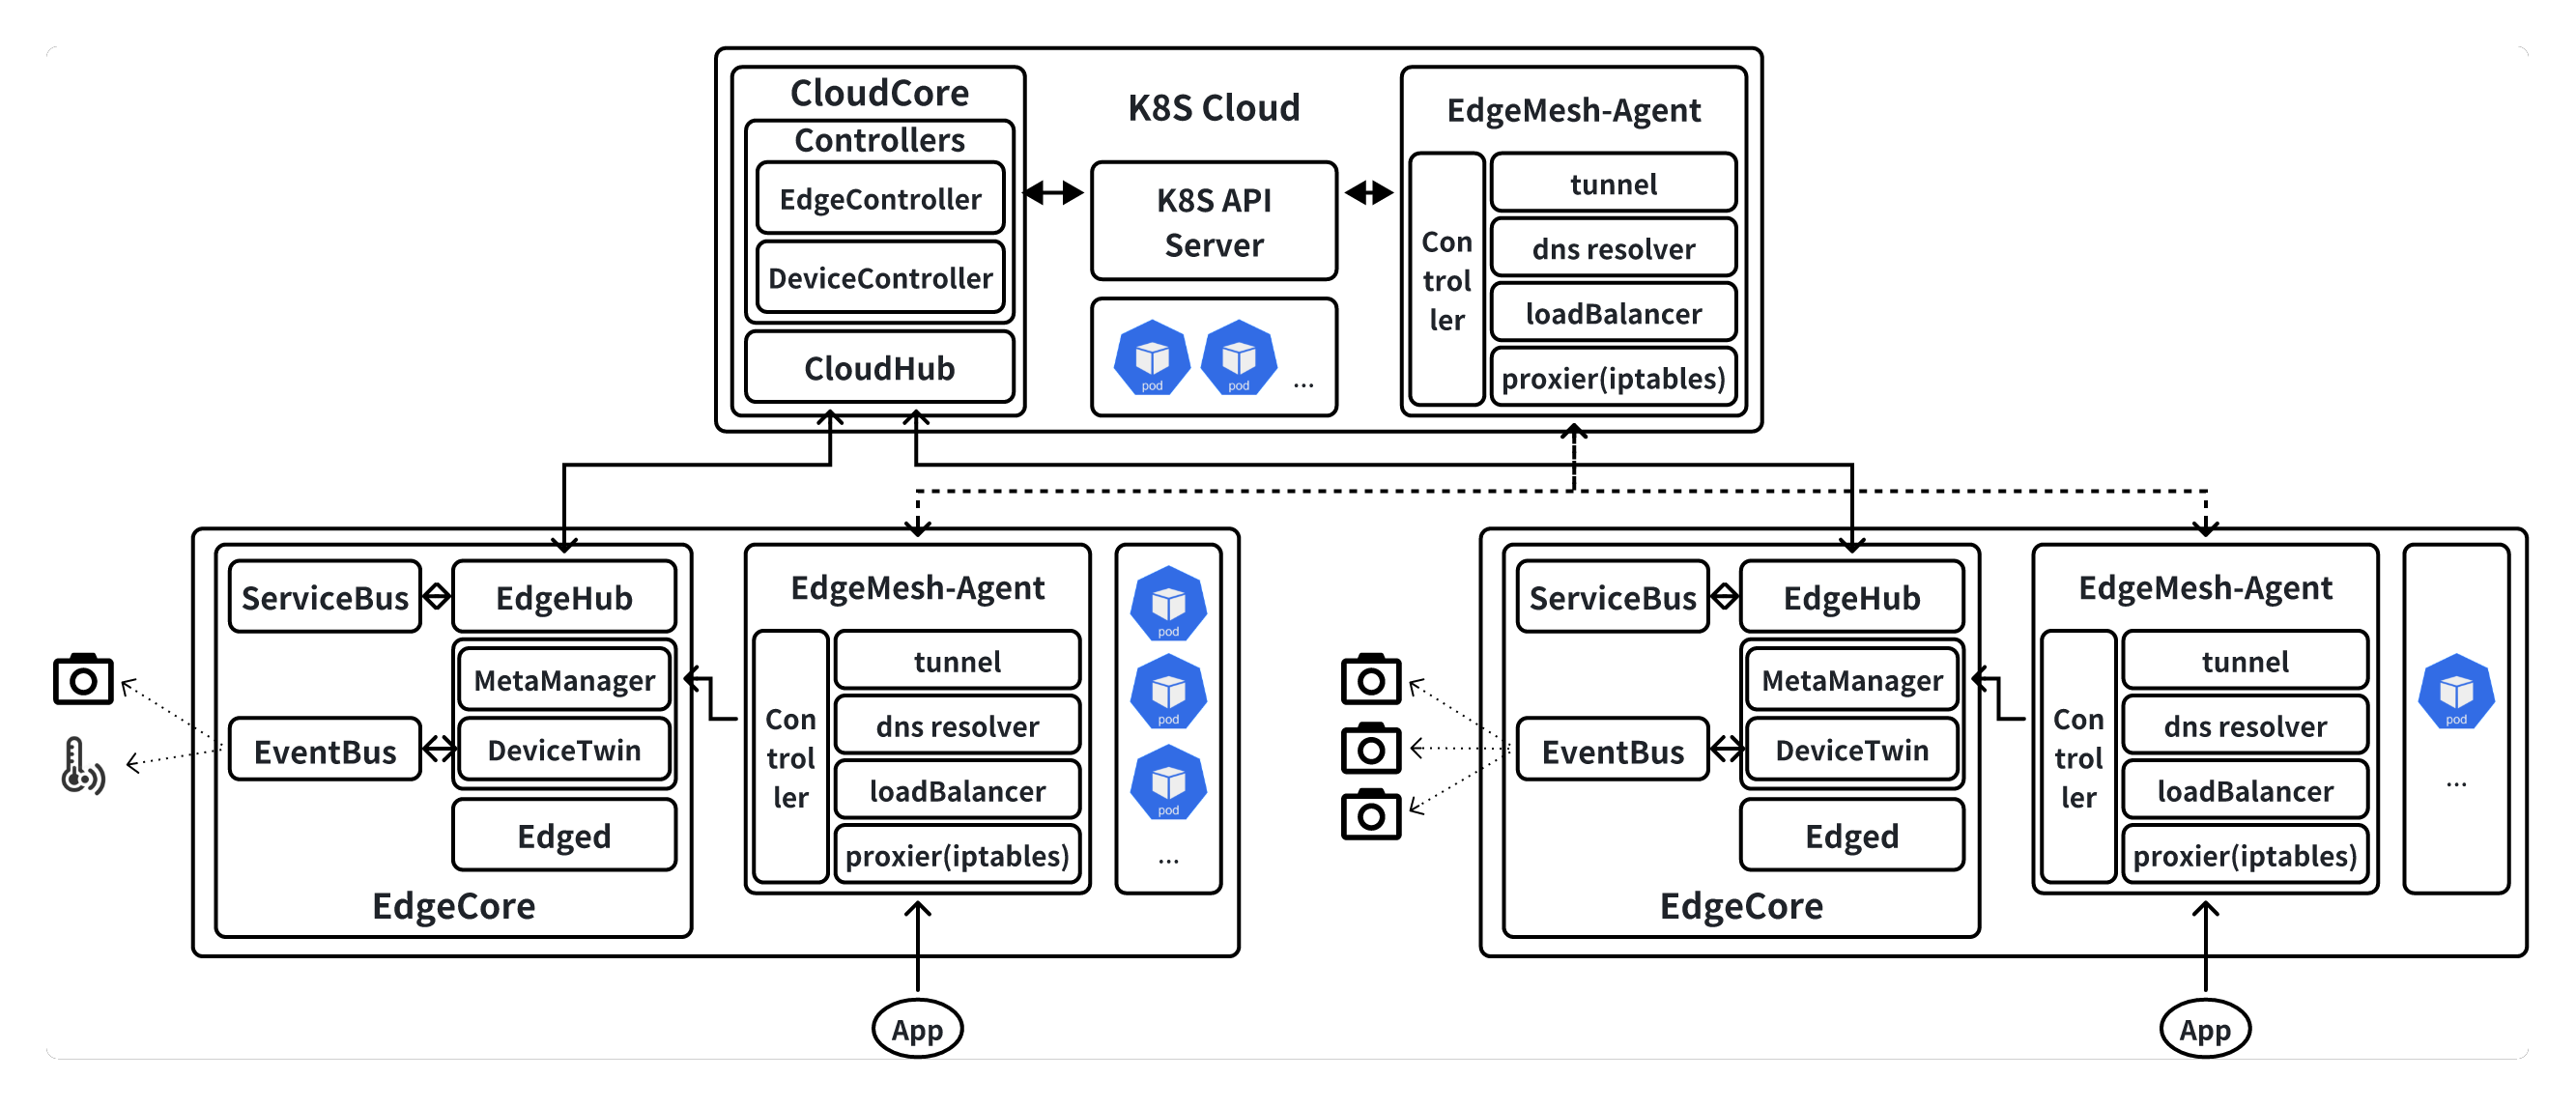
\includegraphics[width=\linewidth]{pics/2-2kubeedge.png}
  \caption{kubeedge的基础架构}
  \label{fig:2-3kubeedge}
\end{figure}

云端核心由控制器(Controller)和 CloudHub 两个组件组成,其中控制器分为边缘控制器(Edge Controller)和设备控制器(Device Controller):边缘控制器负责 Kubernetes API Server 和边缘核心之间的事件同步,而设备控制器专注于物联网设备的管理与更新;CloudHub 则作为控制器与边缘核心之间的通信中介,负责监控云端状态变化、缓存消息,并通过 socket 实现双向通信。

边缘核心主要包括以下五个组件:EdgeD 负责运行和管理基于容器的应用,支持 pod 管理、生命周期事件生成、机密管理、容器运行时支持以及工作负载部署;EdgeHub 负责边缘与云端之间的通信,通过 socket 连接实现资源同步、设备状态更新及消息转发;EventBus 提供 MQTT 客户端交互功能,支持发布/订阅机制;DeviceTwin 用于存储设备状态并同步到云端,同时为应用提供查询接口;MetaManager 作为 EdgeD 和 EdgeHub 之间的消息处理器,负责元数据的存储与检索。

EdgeMesh 是 KubeEdge 集群的数据平面组件,主要提供高可用支持、服务发现和流量代理功能。它利用 LibP2P 技术在边缘节点之间搭建通信网络:对于局域网内的节点,直接访问即可完成数据交互;在跨局域网场景下,则通过打洞隧道技术或中继流量实现数据传输。此外,EdgeMesh 借助 EdgeHub - CloudHub 隧道分发元数据,从而无需直接访问云端,并通过在节点层面部署的 DNS 服务器提升服务搜索的可靠性。在负载均衡方面,EdgeMesh 采用 Istio 的目标规则(DestinationRule),提供轮询和随机等方案,以确保流量在各 Pod 间高效分配,如图 \ref{fig:2-3edgemesh} 所示。

\begin{figure}[ht]
  \centering
  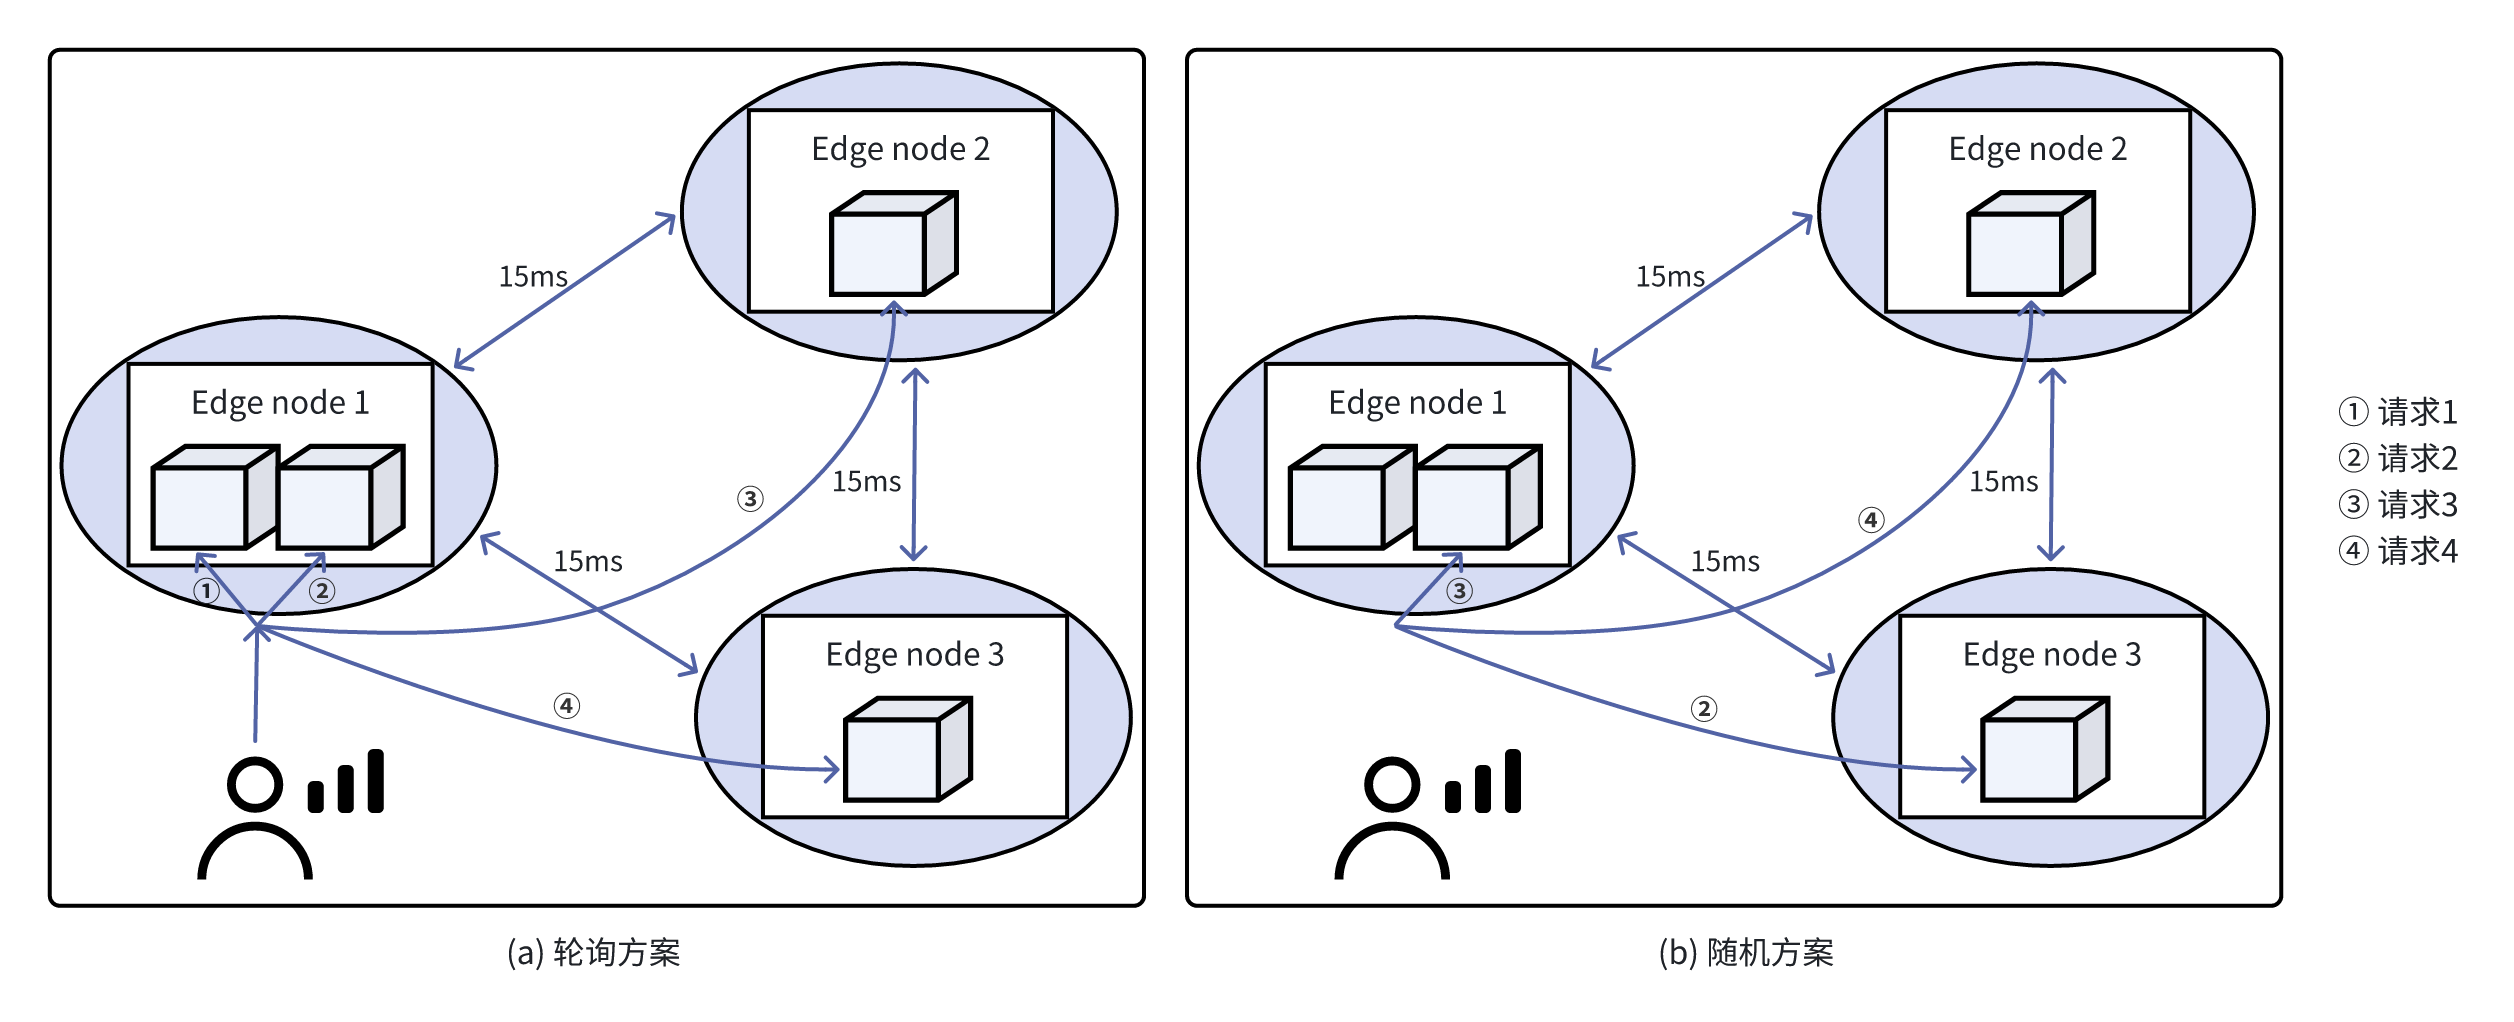
\includegraphics[width=\linewidth]{pics/2-3edgemesh.png}
  \caption{KubeEdge 中的负载均衡方案}
  \label{fig:2-3edgemesh}
\end{figure}

然而,EdgeMesh 并未考虑边缘节点间转发请求所带来的额外延迟。由于边缘计算环境中节点通常地理位置分散,跨节点间的流量转发会显著增加网络时延,降低集群整体吞吐量。针对此问题,Kim 等人\cite{kim2023local}提出了本地调度方案:当边缘节点收到用户请求后,将其平均分配给同一节点上的 Pod,而非转发给远程节点。这样不仅避免了跨节点流量转发导致的高延迟,还能在本地边缘节点即时处理用户请求,从而提升系统的整体吞吐量。然而,本地调度方案也存在不足之处。由于边缘端基础设施通常故障率较高且维护成本较高,当某节点掉线时,部分请求可能无法满足服务质量需求。为解决这些问题,Haja 等人\cite{haja2019sharpening} 提出了 Pod 占位符机制。该机制通过调度算法为每个 Pod 分配一个具有反亲和性(Anti-Affinity)的占位符。当 Pod 所在的主机节点发生故障时,占位符可以迅速在符合延迟约束的其他节点上重新启动 Pod,从而确保服务的连续性。但是,该方法主要关注单节点的可靠性,未能充分利用分布式边缘节点之间的协同能力,限制了系统在高负载场景下的扩展性和整体可靠性。

KubeEdge 的负载 Pod 调度过程依赖于云端 Kubernetes 的调度机制,如图 \ref{fig:2-4k8sschedule} 所示。云端的 Kubernetes 调度器(kube-scheduler)通过监听未分配节点的 Pod,采用两步法选择最佳节点:首先,通过过滤(Filtering)策略(如资源需求、亲和性、反亲和性等),排除不符合条件的节点,生成可行节点列表;接着,通过打分(Scoring)策略(如资源平衡、数据本地性等),对可行节点进行评分,并选择得分最高的节点。如果存在多个得分相同的节点,则随机选择一个进行绑定。

\begin{figure}[ht]
  \centering
  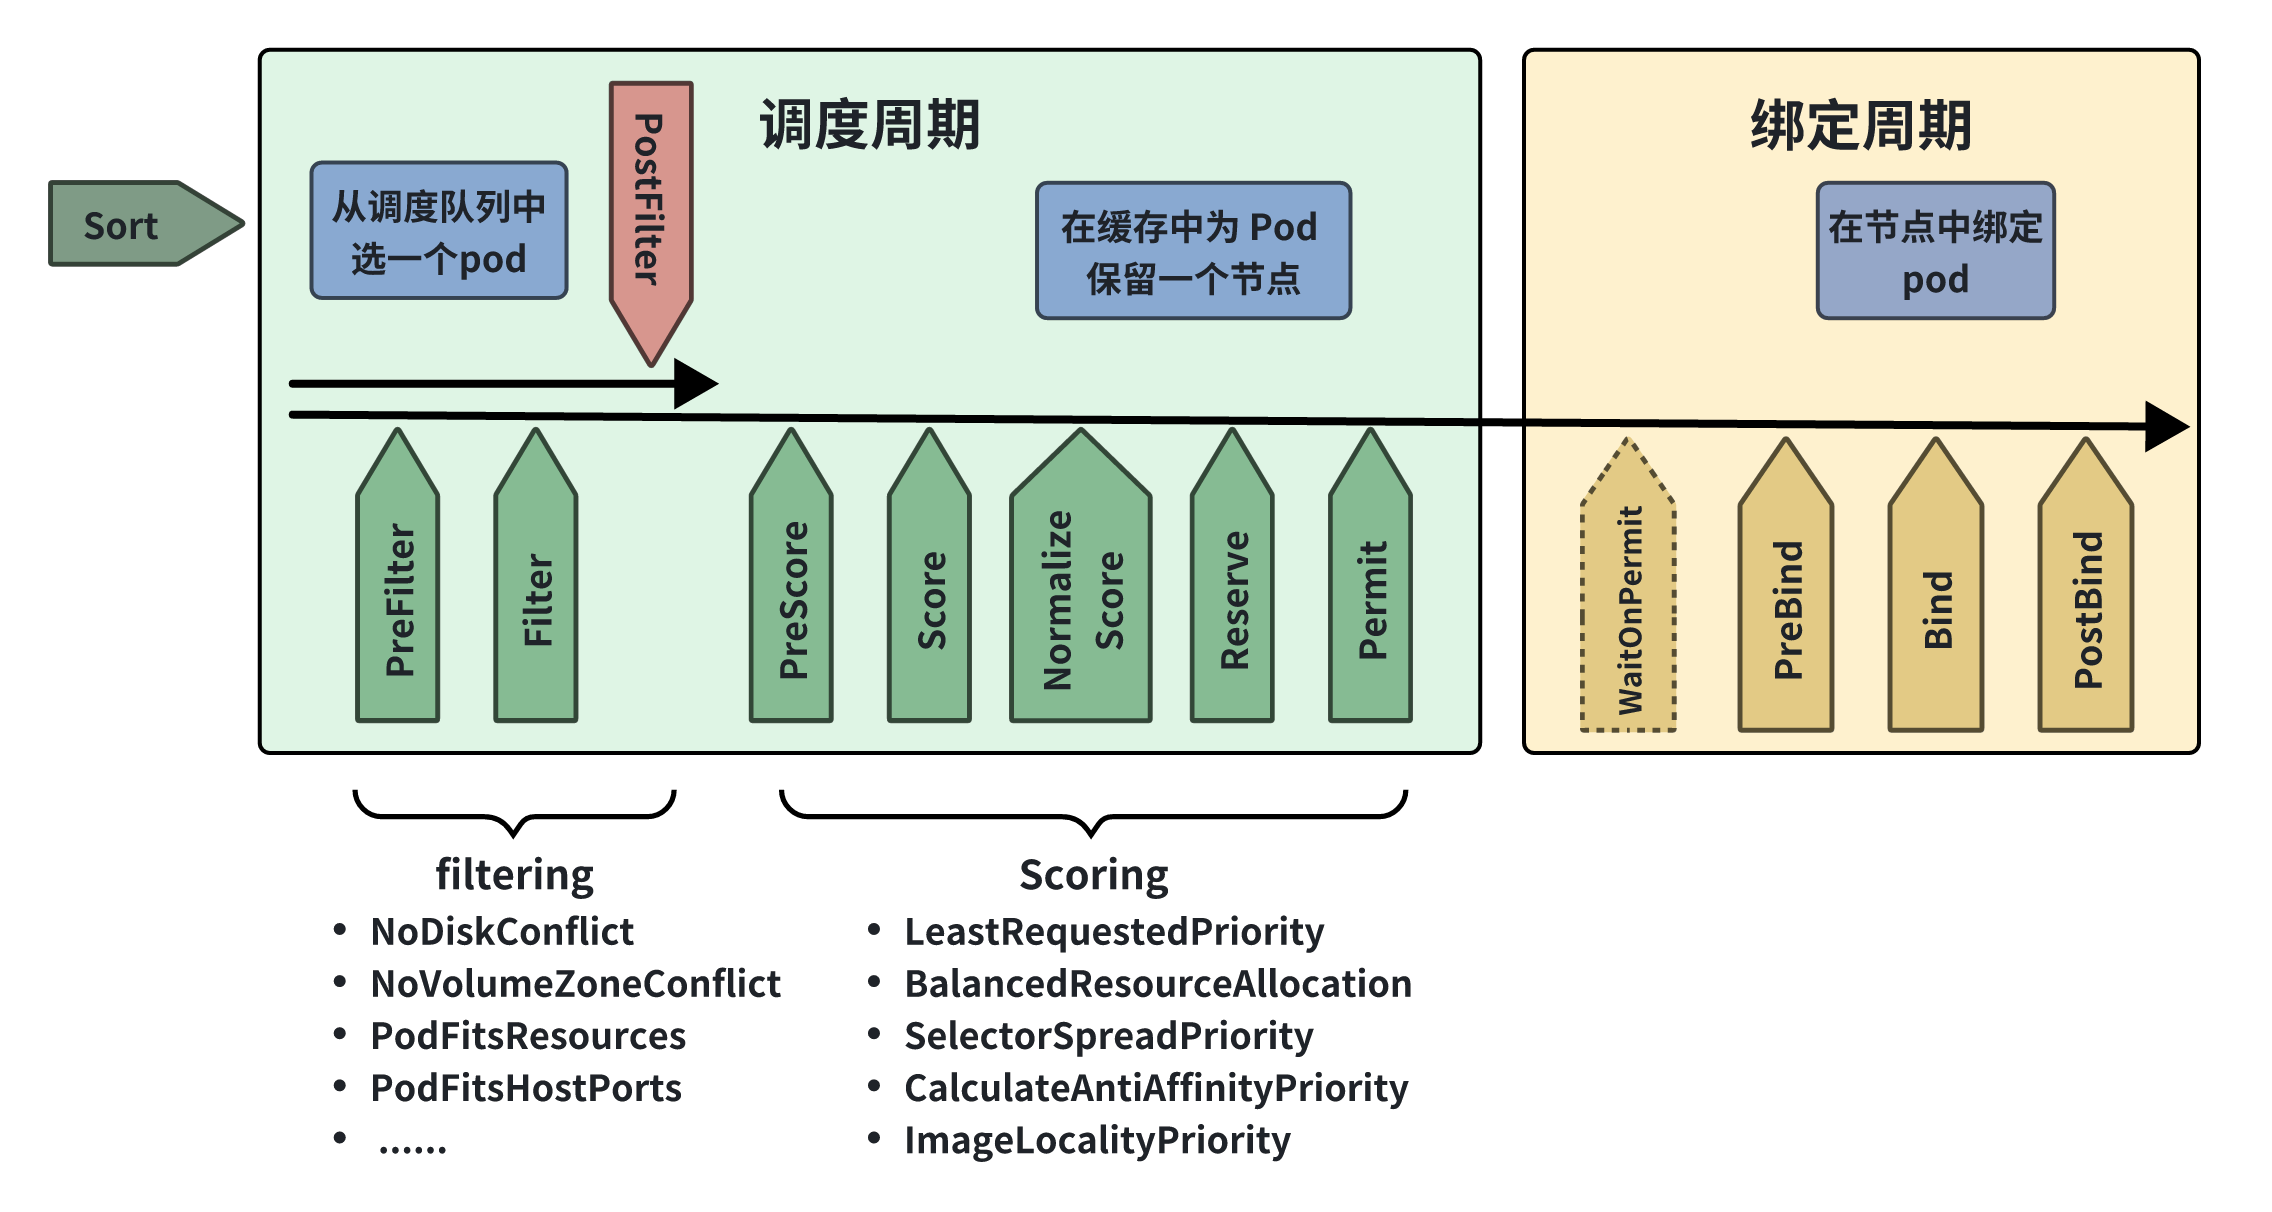
\includegraphics[width=\linewidth]{pics/2-4k8sschedule.png}
  \caption{Kubernetes 中的负载调度方案}
  \label{fig:2-4k8sschedule}
\end{figure}

然而,Kubernetes 的调度逻辑主要针对云端高性能节点设计,在边缘环境中存在适配性不足的问题,面临资源协调与应用协作管理的双重挑战。在资源协调方面,云边网络具有松散耦合的结构和较高的通信时延,导致云端调度器难以及时掌握边缘资源的实时利用率,从而无法在最佳时机完成任务的优化调度。在应用协作方面,现有云端调度机制对用户服务质量的感知和支持不足,难以有效应对云边协同应用中任务的垂直卸载和水平迁移需求,这进一步增加了应用协作管理的复杂性。

为了解决上述问题,Lingayya 等人\cite{lingayya2024dynamic} 提出了一种创新的资源管理与任务调度方案,旨在提高边缘计算环境的适应性和运行效率。该方案在边缘节点部署高效的监测模块,实时采集设备资源状态(包括计算能力、内存使用、网络带宽等)和任务队列信息,同时利用多智能体协同强化学习方法,通过多个智能体在共享环境中协作,综合各自的目标和能力,优化整体系统性能。此外,Shan 等人\cite{shan2024kces} 提出了一种资源分配算法。当资源评估结果显示当前节点无法满足任务需求时,该算法通过动态调整任务的资源分配方案,使节点能够容纳更多任务,同时确保任务的最小资源需求,从而最大化资源利用率。如果调整后资源仍无法满足需求,则通过任务水平迁移,将任务分配到其他边缘节点。此外,该方案结合设备的监控模式,对任务进行合理卸载,选择合适的边缘节点或云节点执行,从而实现云边协同的垂直卸载。然而,上述方案主要面向通用负载,对深度学习模型的适配能力较低,难以以低成本高效地获取负载的运行时延,仍存在一定的改进空间。

\section{边缘端节点监测技术}

边缘端通常由多种类型的节点组成,包括硬件配置各异的设备和具有不同网络带宽与延迟特性的连接\cite{cooke2020model,varghese2021survey,barbalace2020edge}。例如,这些节点可能配备低功耗的 CPU、高并行处理能力的多核 GPU,或专用的 AI 加速器(如 VPU)等硬件资源。这种硬件和网络特性的异构性导致节点在计算能力、存储容量和能耗限制上存在显著差异,从而显著增加了资源分配与利用优化的复杂性。

\subsection{边缘端节点推理能力监测技术}

对于深度学习推理来说,模型的计算需求必须适配目标设备的硬件特性,但异构环境下的适配和模型迁移需要对任务进行细粒度划分和动态调整,从而大幅增加了调度的复杂性。在边缘端,评估深度学习推理性能的关键指标是推理时延。传统的基于测量的方法需要复杂的部署过程,尤其在多样化的边缘设备和推理框架场景下,难以应对设备数量的快速增长。现有的基于FLOPs的方法在预测准确性上存在不足,无法满足实际需求。

为了解决这一问题,Zhang 等人\cite{zhang2021nn} 提出了 nn-Meter 工具,如图 \ref{fig:2-5nnmeter} 所示。该工具通过设计测试用例,自动检测模型在不同边缘设备上的推理执行单元(内核),并基于检测到的融合规则,递归地将模型划分为内核,从而有效捕获不同设备上的算子融合行为,大幅提高了预测的准确性。nn-Meter 的核心技术包括以下几个方面:首先,根据模型设计和硬件延迟特性对内核配置进行剪枝;其次,通过迭代采样过程自动选择最优配置进行检测,而非采用随机选择策略;最后,利用机器学习回归器学习采样数据的非线性关系,构建高效的内核级延迟预测器。这一方法显著降低了数据采样成本,同时大幅提高了预测准确性。在 nn-Meter 工具的基础上,本文进一步对其进行了改进,使其适配云原生环境,能够在不同资源隔离策略下进行推理时延预测。通过这些改进,系统不仅能够满足多样化边缘设备的性能评估需求,还能够更好地支持云边协同环境下的推理任务优化。

\begin{figure}[ht]
  \centering
  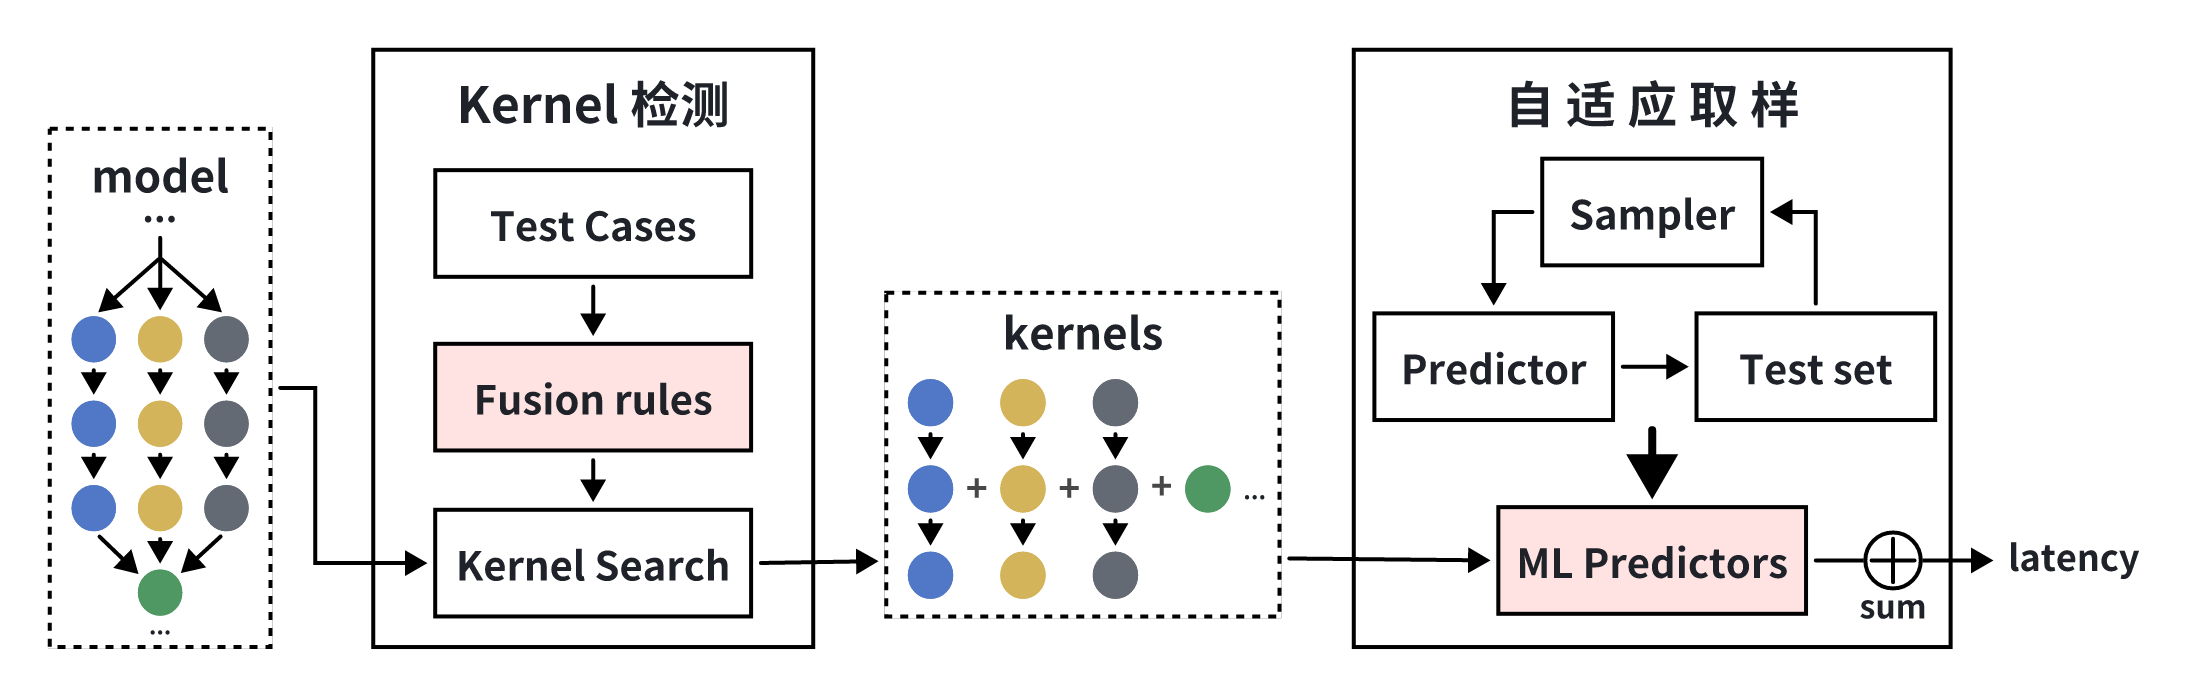
\includegraphics[width=\linewidth]{pics/2-5nnmeter.png}
  \caption{nn-Meter工具的架构}
  \label{fig:2-5nnmeter}
\end{figure}

\subsection{边缘端节点间通信监测技术}

边缘端节点通常分布在异构网络环境中,其通信性能容易受到网络带宽、延迟、丢包率以及通信协议开销等多种因素的影响。为了解决这一问题,Haja 等人\cite{haja2019sharpening} 提出了一种实时监测边缘节点间传输时延的方法。该方法在每个节点上部署测量 Pod,这些 Pod 定期发送 ping 包并记录往返时间,从而生成延迟数据,如图 \ref{fig:2-6ping} 所示。此设计能够提供实时的通信性能评估,为动态优化和调度策略的制定提供数据支持。

\begin{figure}[ht]
  \centering
  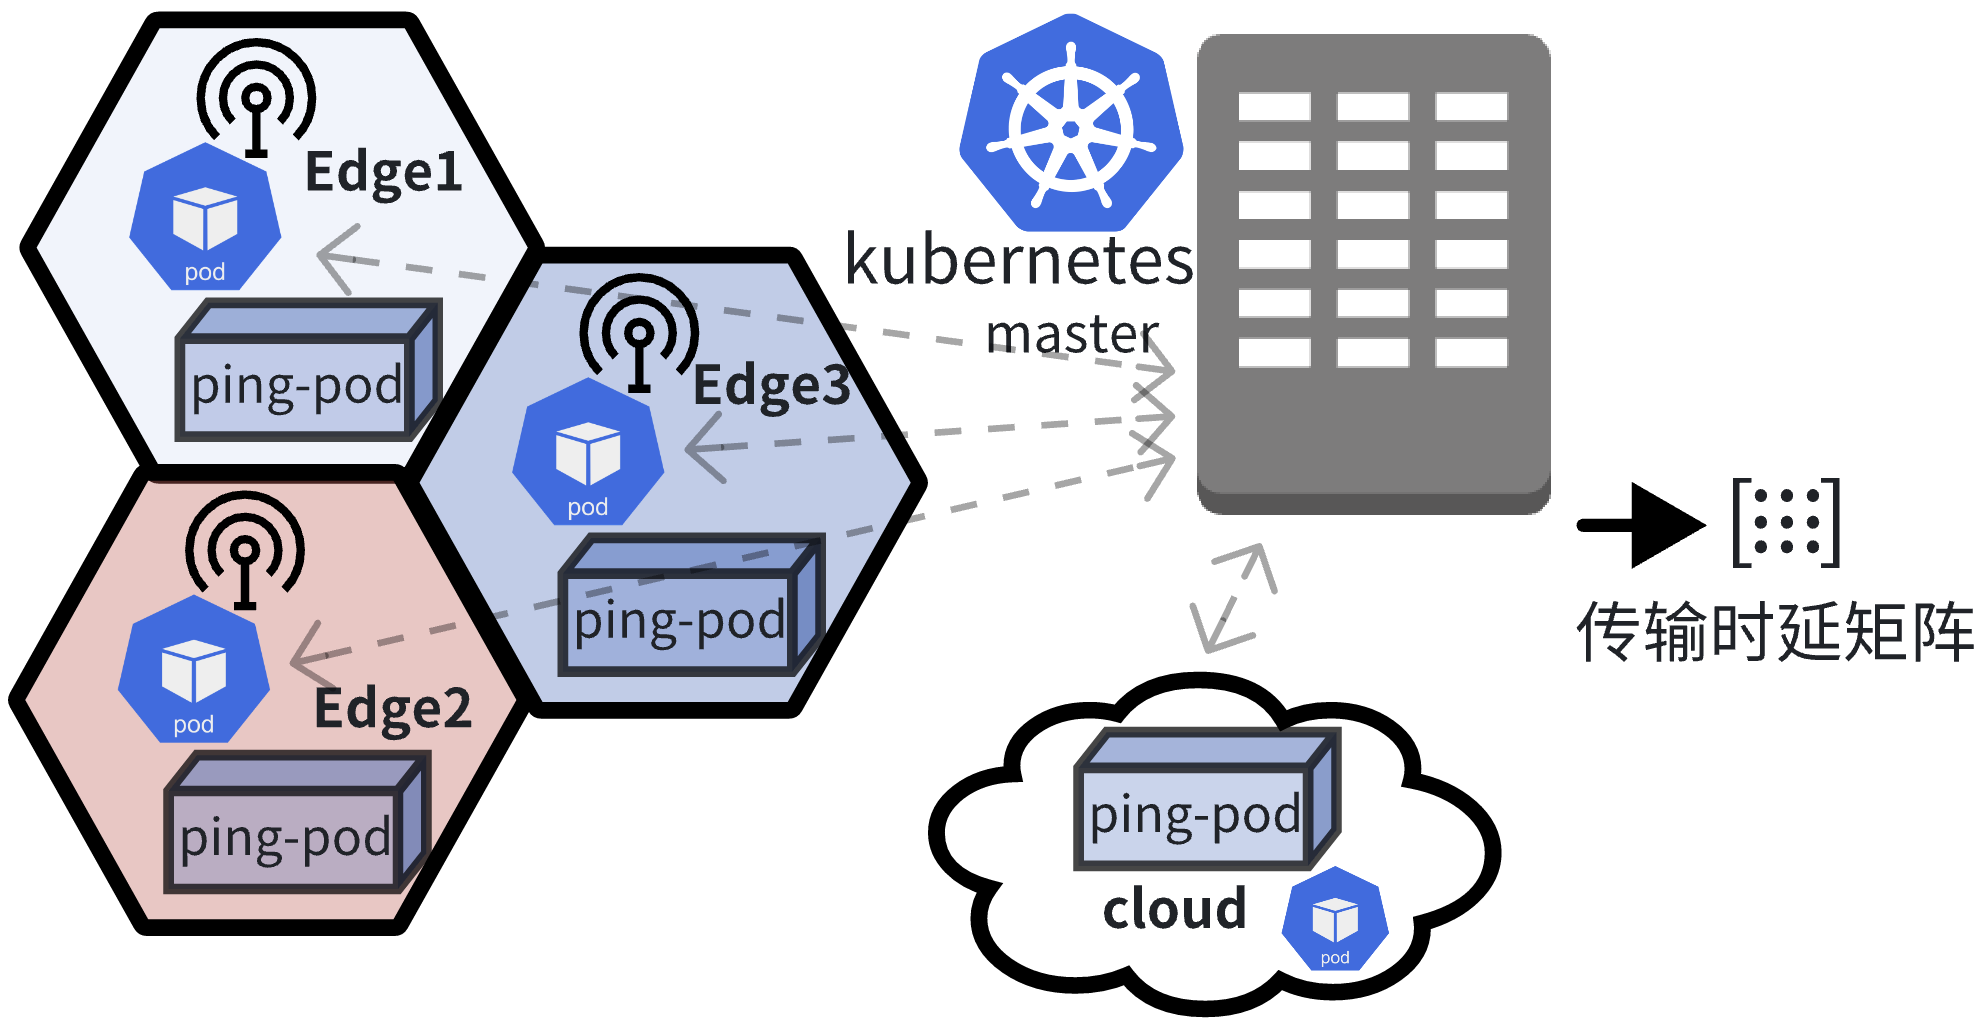
\includegraphics[width=0.7\linewidth]{pics/2-6ping.png}
  \caption{测量并记录传输时延矩阵的过程}
  \label{fig:2-6ping}
\end{figure}

在边缘节点间通信监测中,Ping、iperf3 和 Prometheus + Blackbox Exporter 是三种常用的技术方案,各有其特点和适用场景。Ping 是一种轻量级工具,通过发送 ICMP 请求快速检测网络连通性和往返延迟(RTT),适用于实时性要求高的基础连通性监测,但其功能较为单一,无法提供带宽等深入的性能数据。相比之下,iperf3 提供更详尽的网络性能指标,包括带宽、抖动和丢包率,支持 TCP 和 UDP 协议,适合需要深入分析网络质量的场景。然而,iperf3 的部署较为复杂,且因其占用较多网络资源,不适合实时或生产环境的持续监测。Prometheus + Blackbox Exporter 专注于大规模分布式系统的长期监控,通过周期性探测提供延迟和可用性等性能数据,同时支持多种协议的探测和丰富的数据分析功能,但其配置复杂且在实时性要求较高的场景中可能存在一定延迟。

\section{本章小结}

本章首先系统性地阐述了云边协同的基本概念及其分层架构,并聚焦于云边协同中深度学习推理服务的供应问题,回顾了现有的云端和边缘端推理服务解决方案。随后,详细介绍了本文原型系统所依托的 KubeEdge 架构及其主要服务功能。最后,针对边缘端节点的异构性和复杂性,系统梳理了推理能力监测与通信性能监测技术的最新进展。通过对以上内容的总结,本章不仅为后续研究提供了必要的背景知识和技术支撑,还明确了云边协同在深度学习推理服务中的关键挑战及其潜在解决路径。

